\section{Appendix}

\begin{figure*}[!htb]
	\centering
	% \hspace*{-5mm}
	\subfloat[]{
		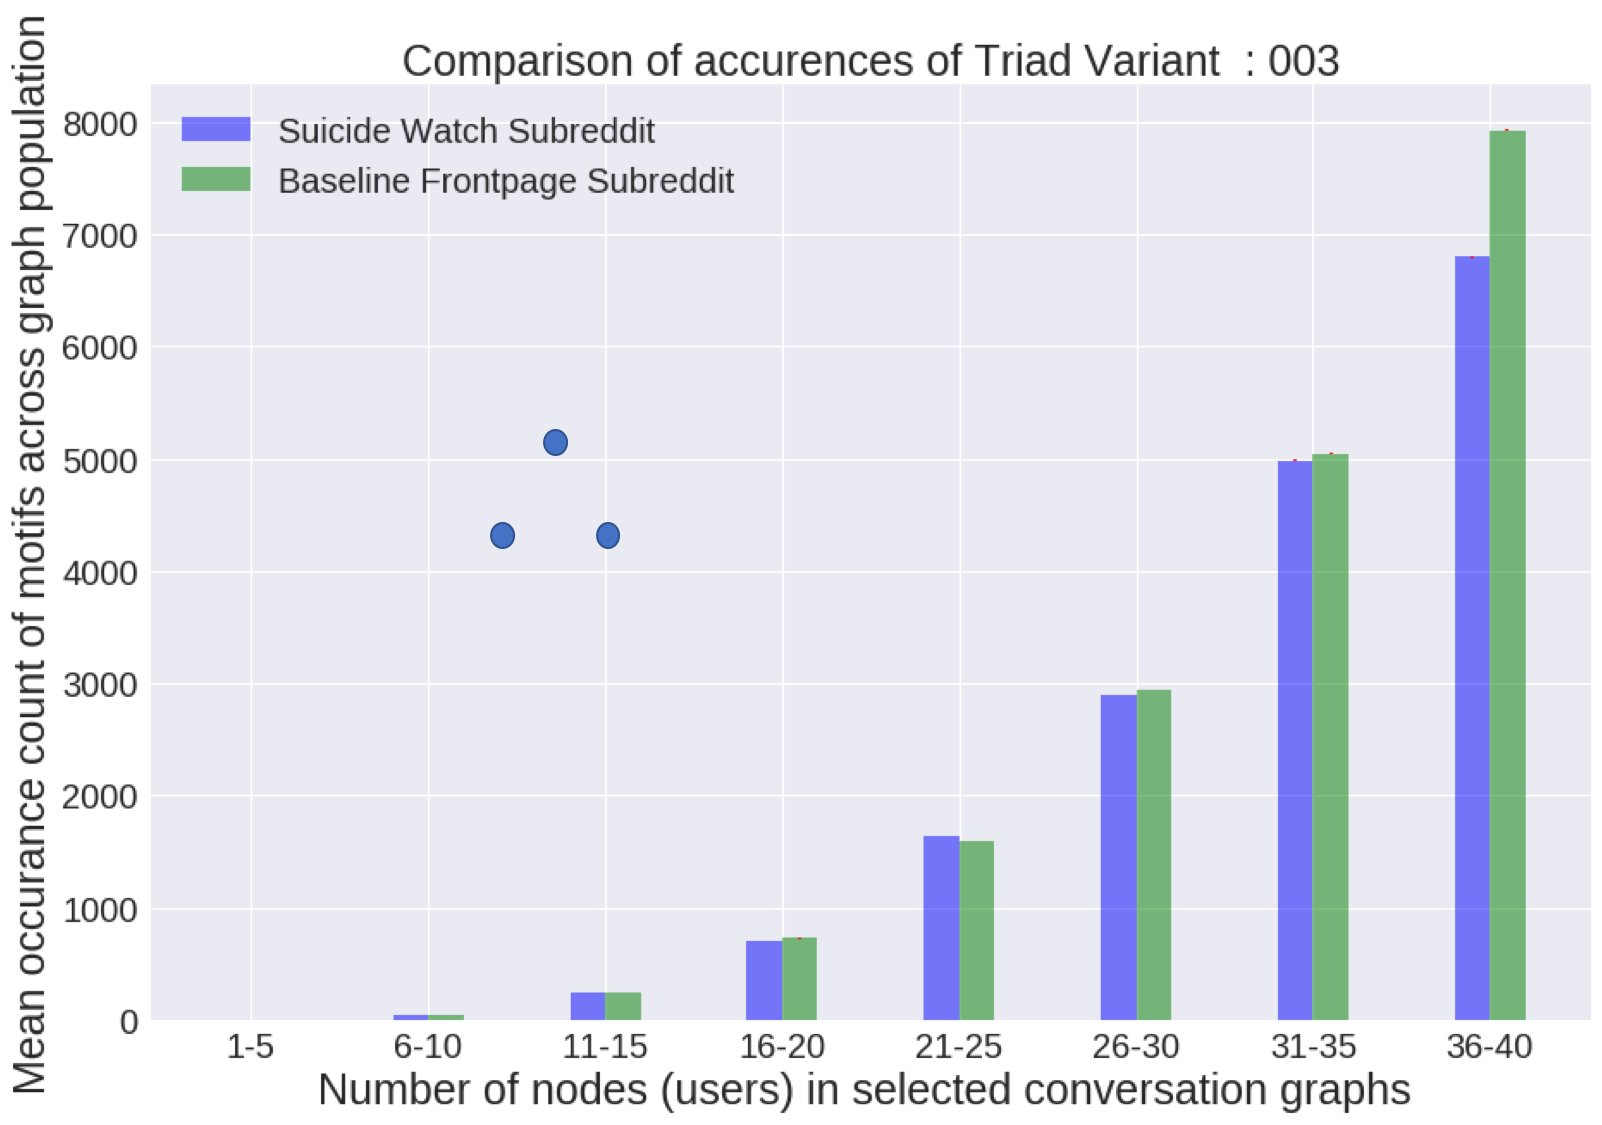
\includegraphics[width=0.33\textwidth, height = 4.5cm ]{Figures/003}
		\label{fig:003}
	}
	\subfloat[]{
		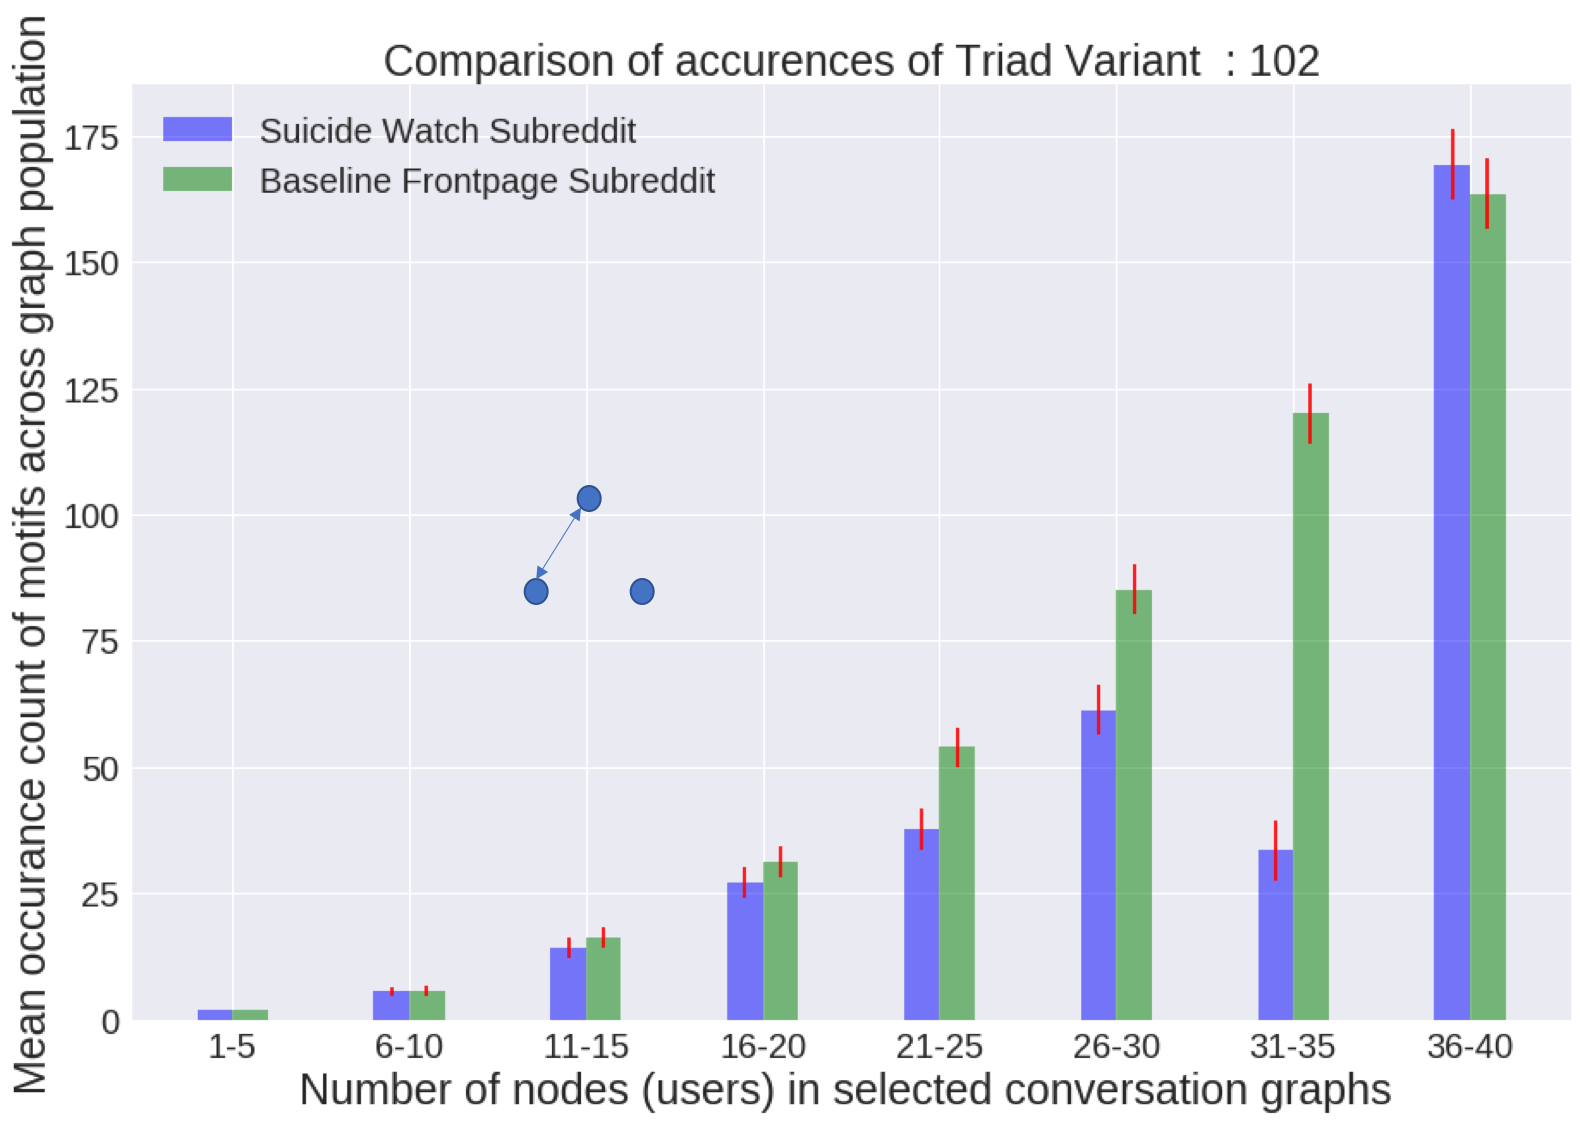
\includegraphics[width=0.33\textwidth, height = 4.5cm ]{Figures/102}
		\label{fig:102}
	}
	\subfloat[]{
		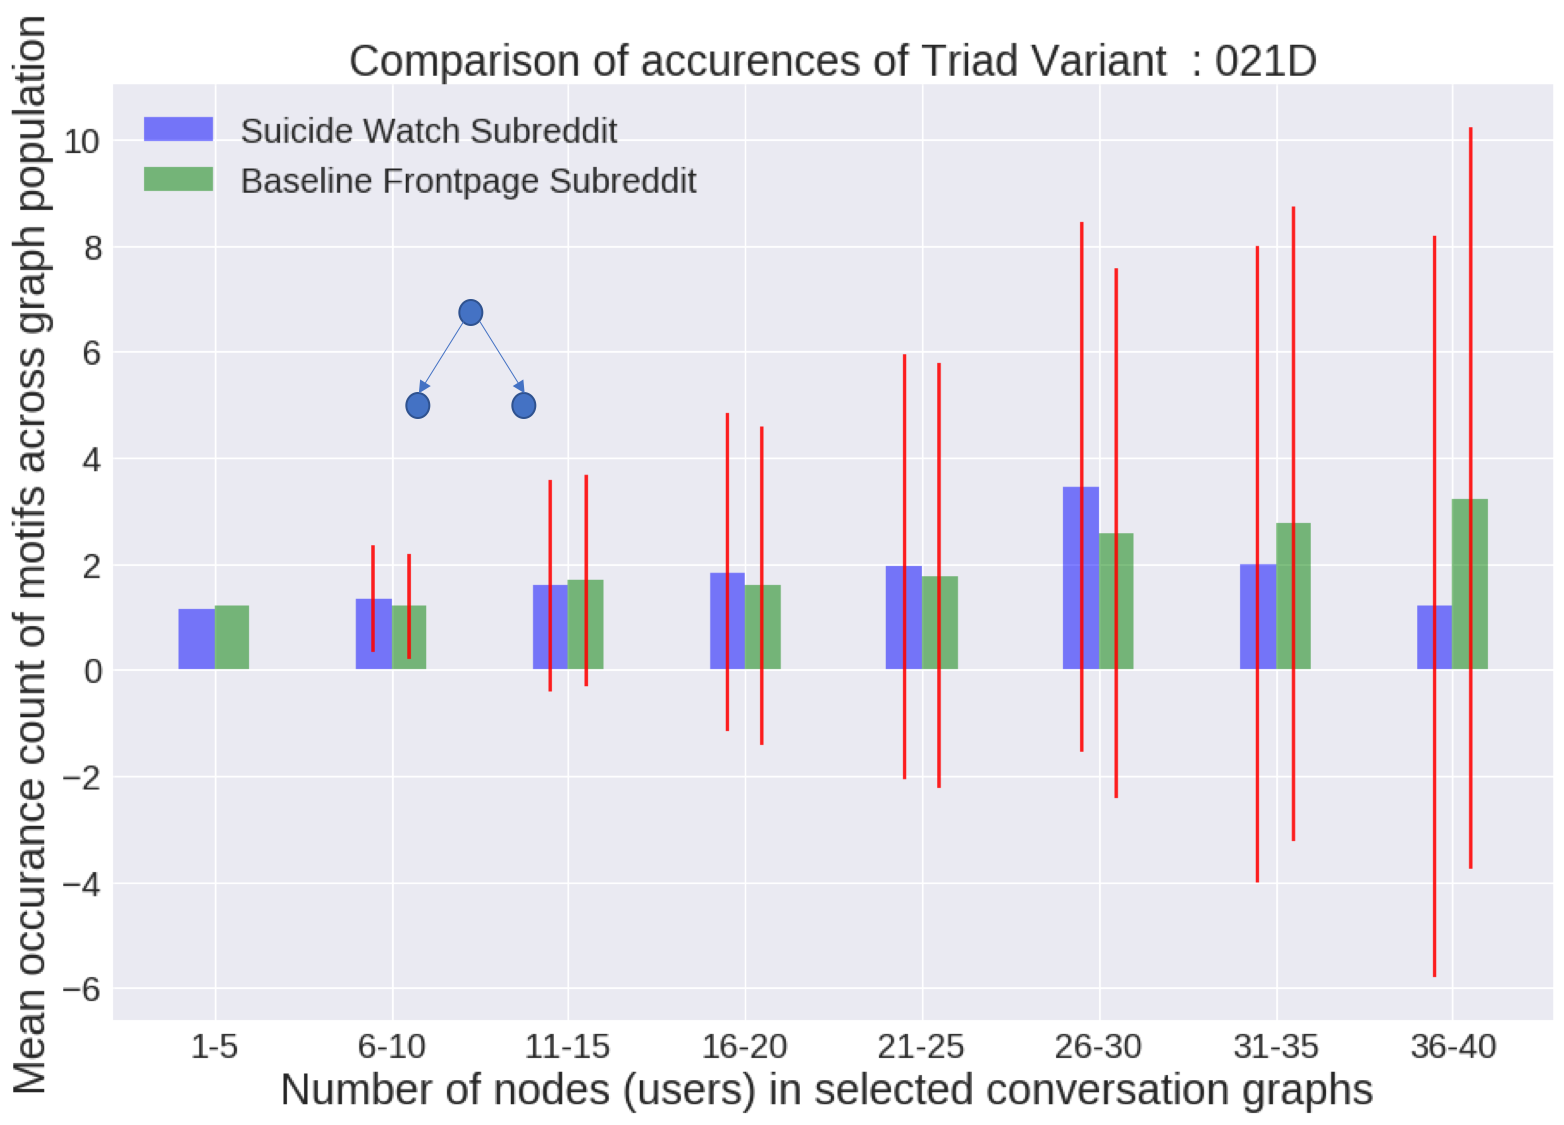
\includegraphics[width=0.33\textwidth, height = 4.5cm ]{Figures/021D}
		\label{fig:021D}
	}


	\subfloat[]{
	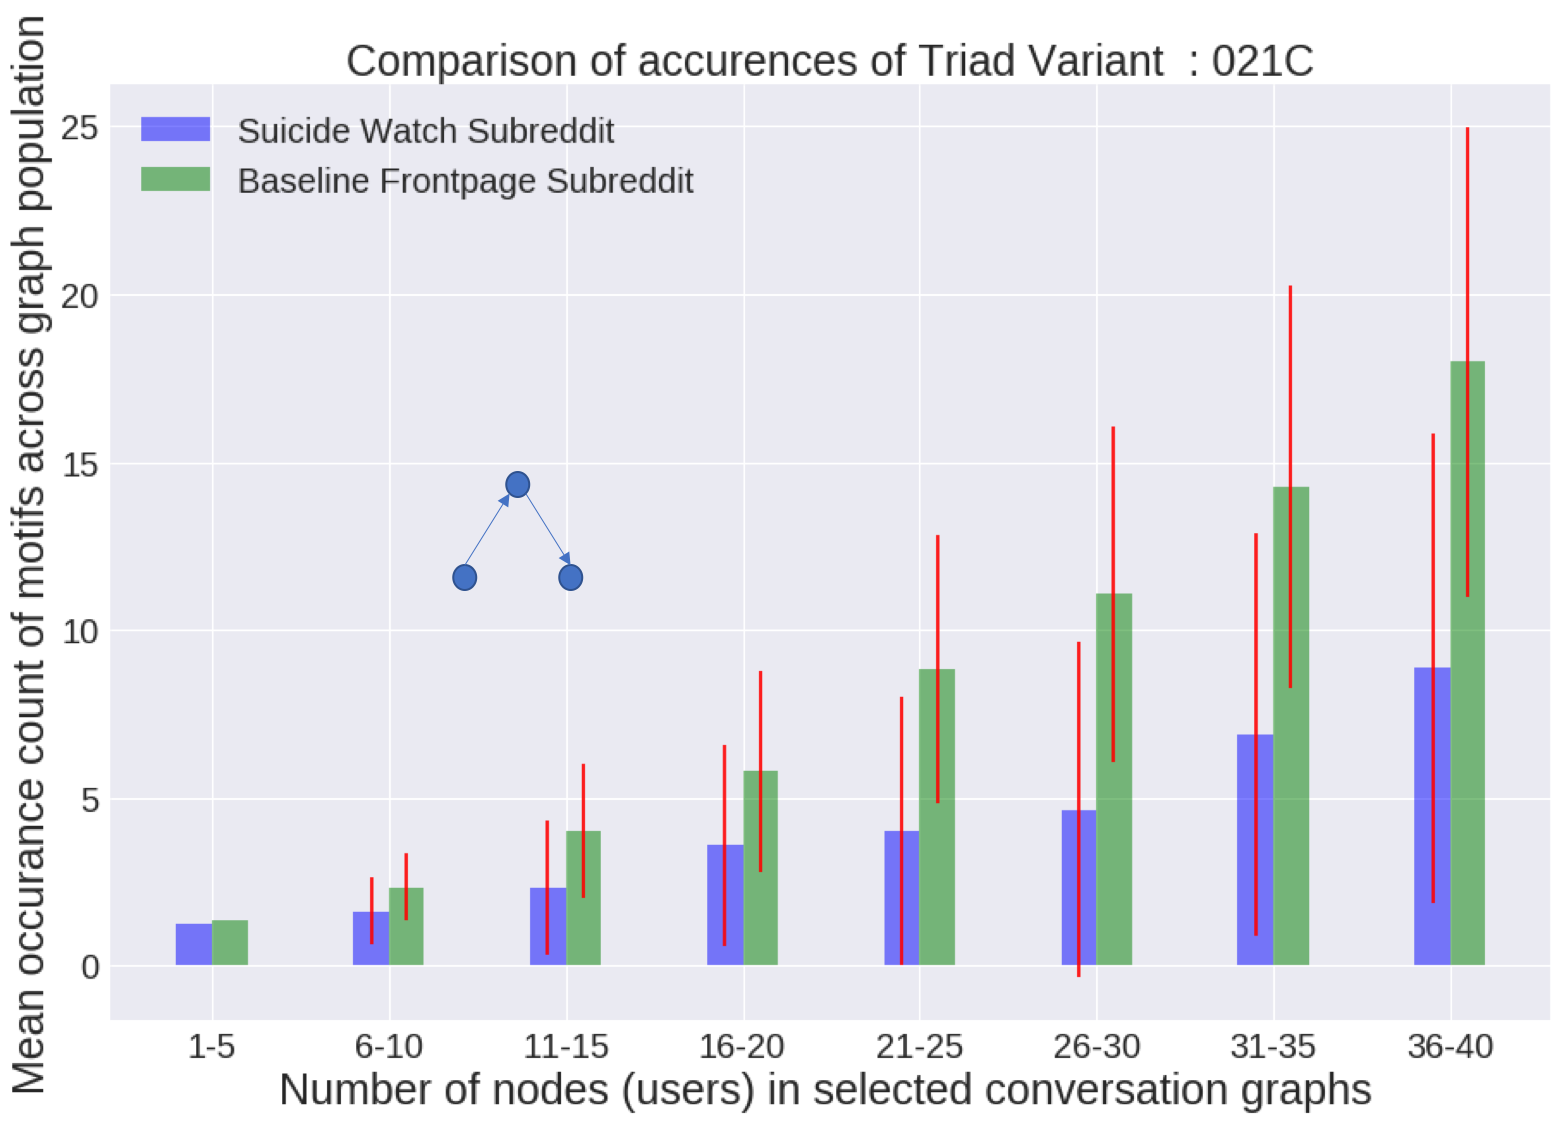
\includegraphics[width=0.33\textwidth, height = 4.5cm ]{Figures/021C}
	\label{fig:021C}
	}
	\subfloat[]{
	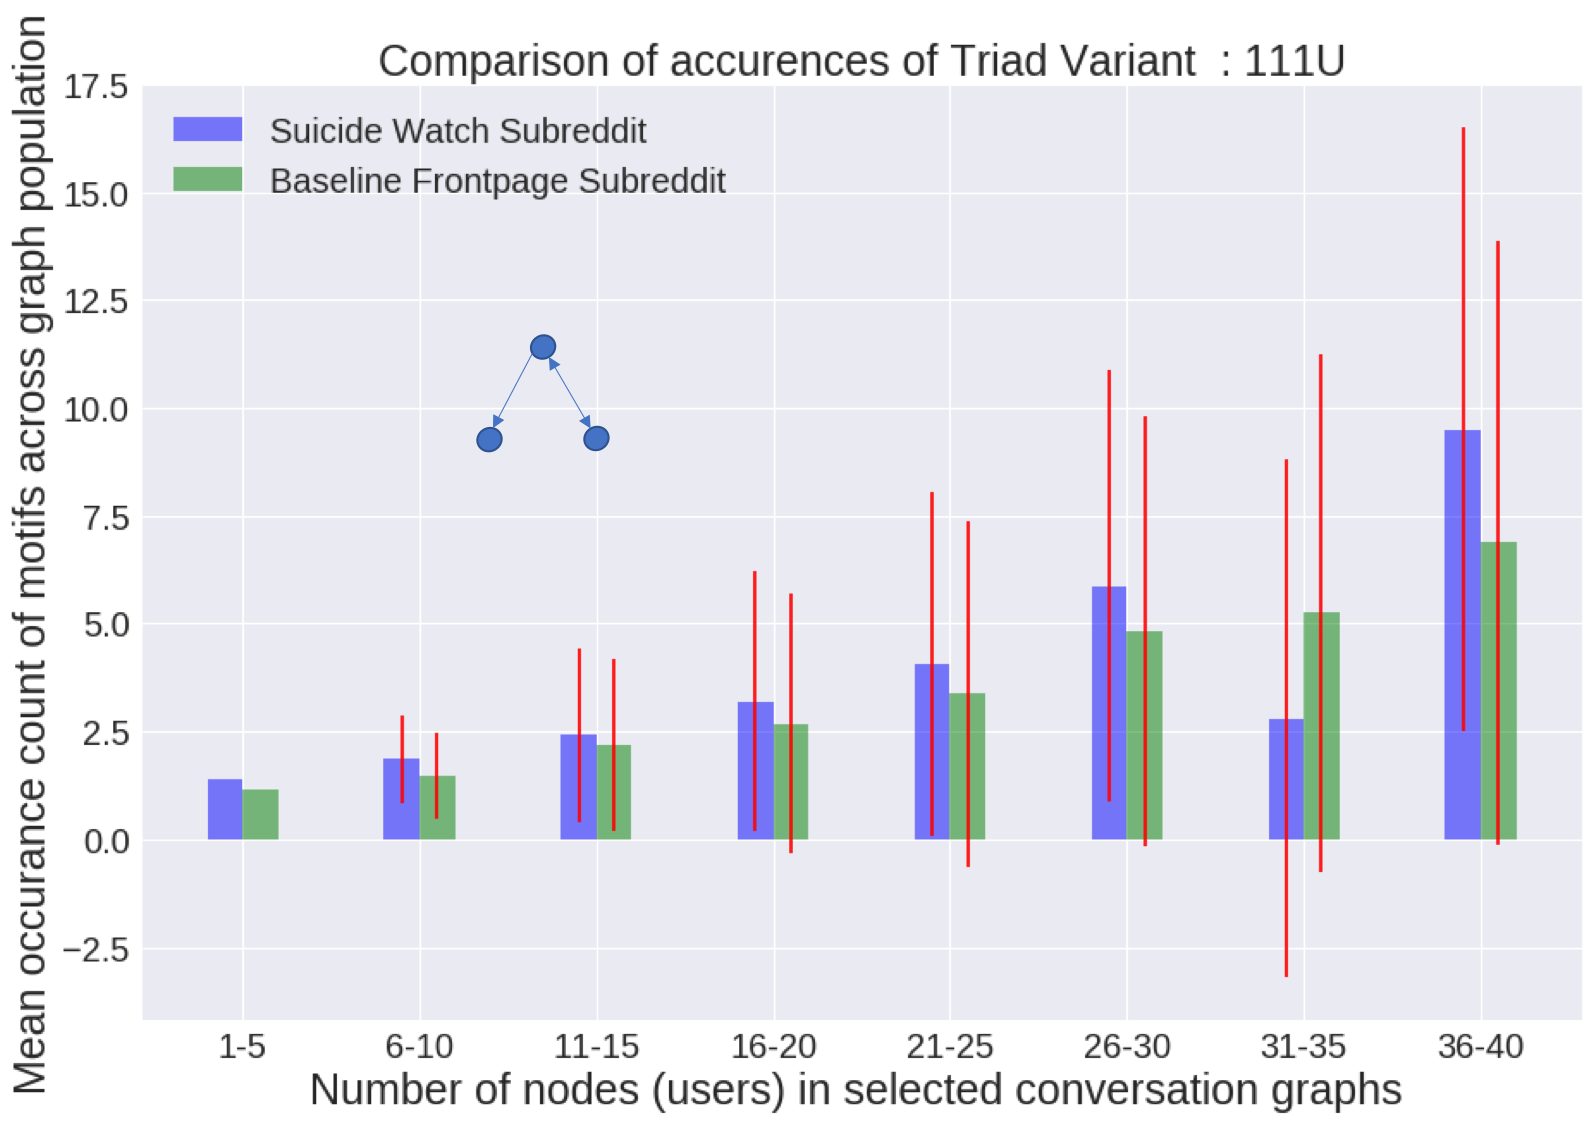
\includegraphics[width=0.33\textwidth, height = 4.5cm ]{Figures/111U}
	\label{fig:111U}
	}
    \subfloat[]{
	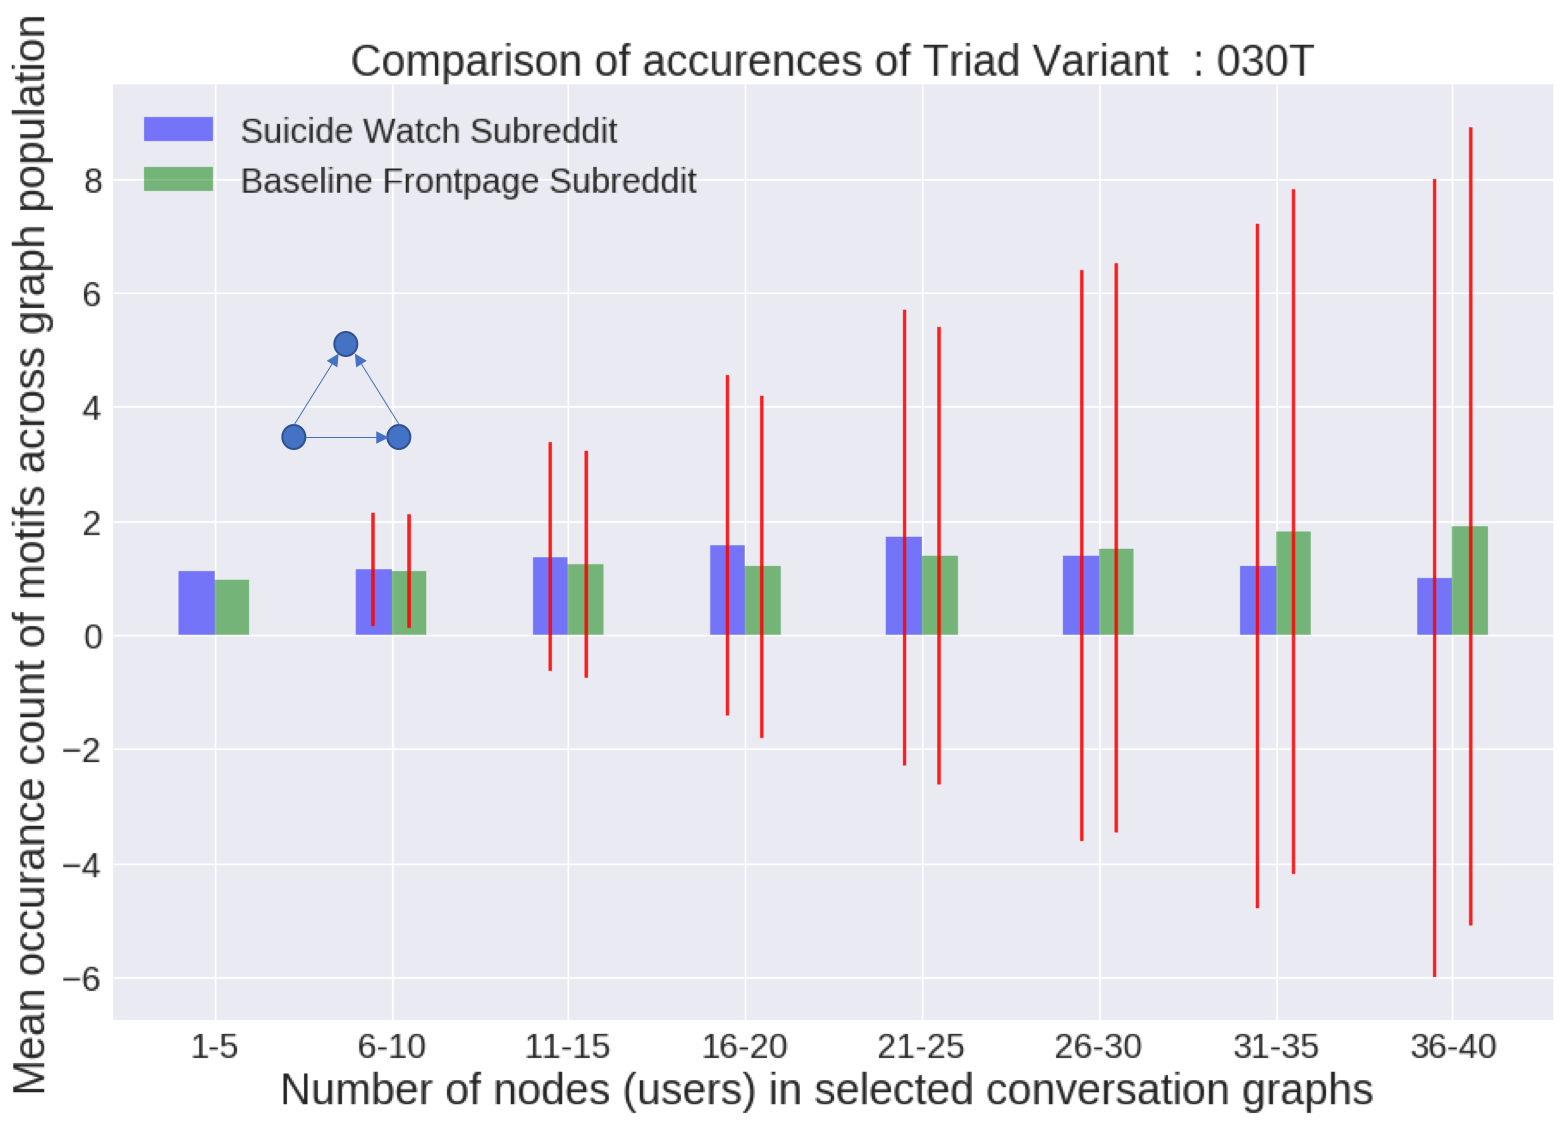
\includegraphics[width=0.33\textwidth, height = 4.5cm ]{Figures/030T}
	\label{fig:030T}
	}
	
    \subfloat[]{
	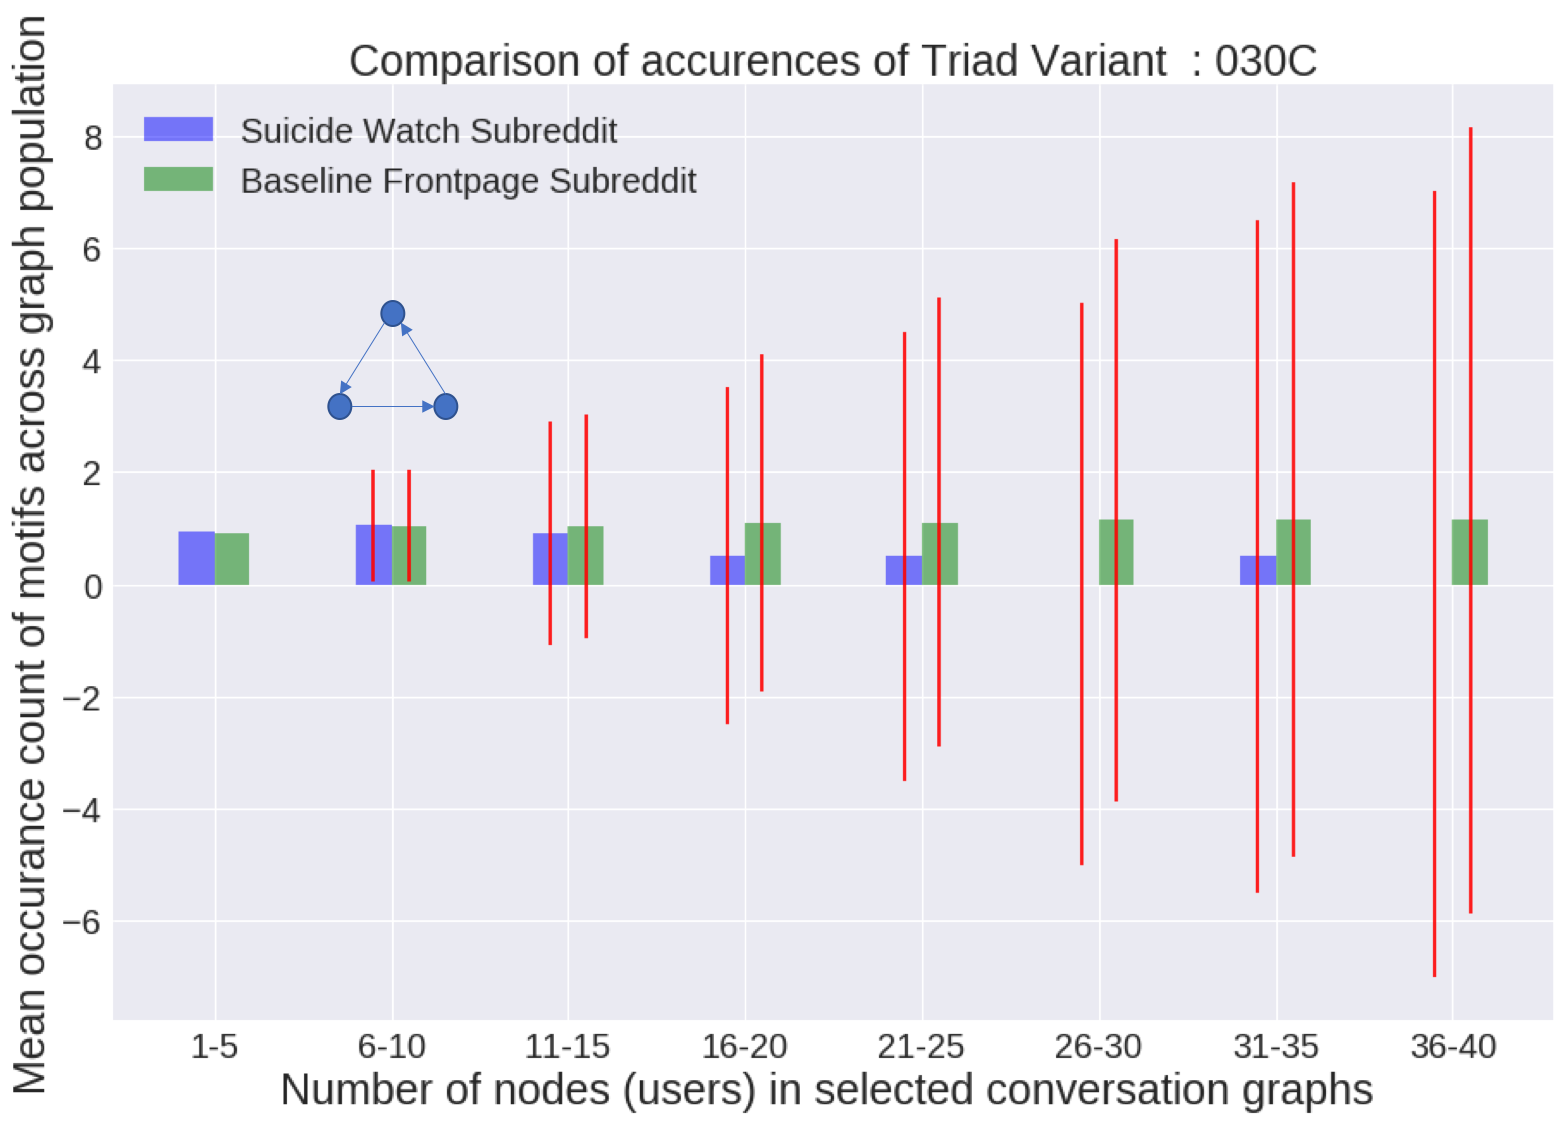
\includegraphics[width=0.33\textwidth, height = 4.5cm ]{Figures/030C}
	\label{fig:030C}
	}
	\subfloat[]{
	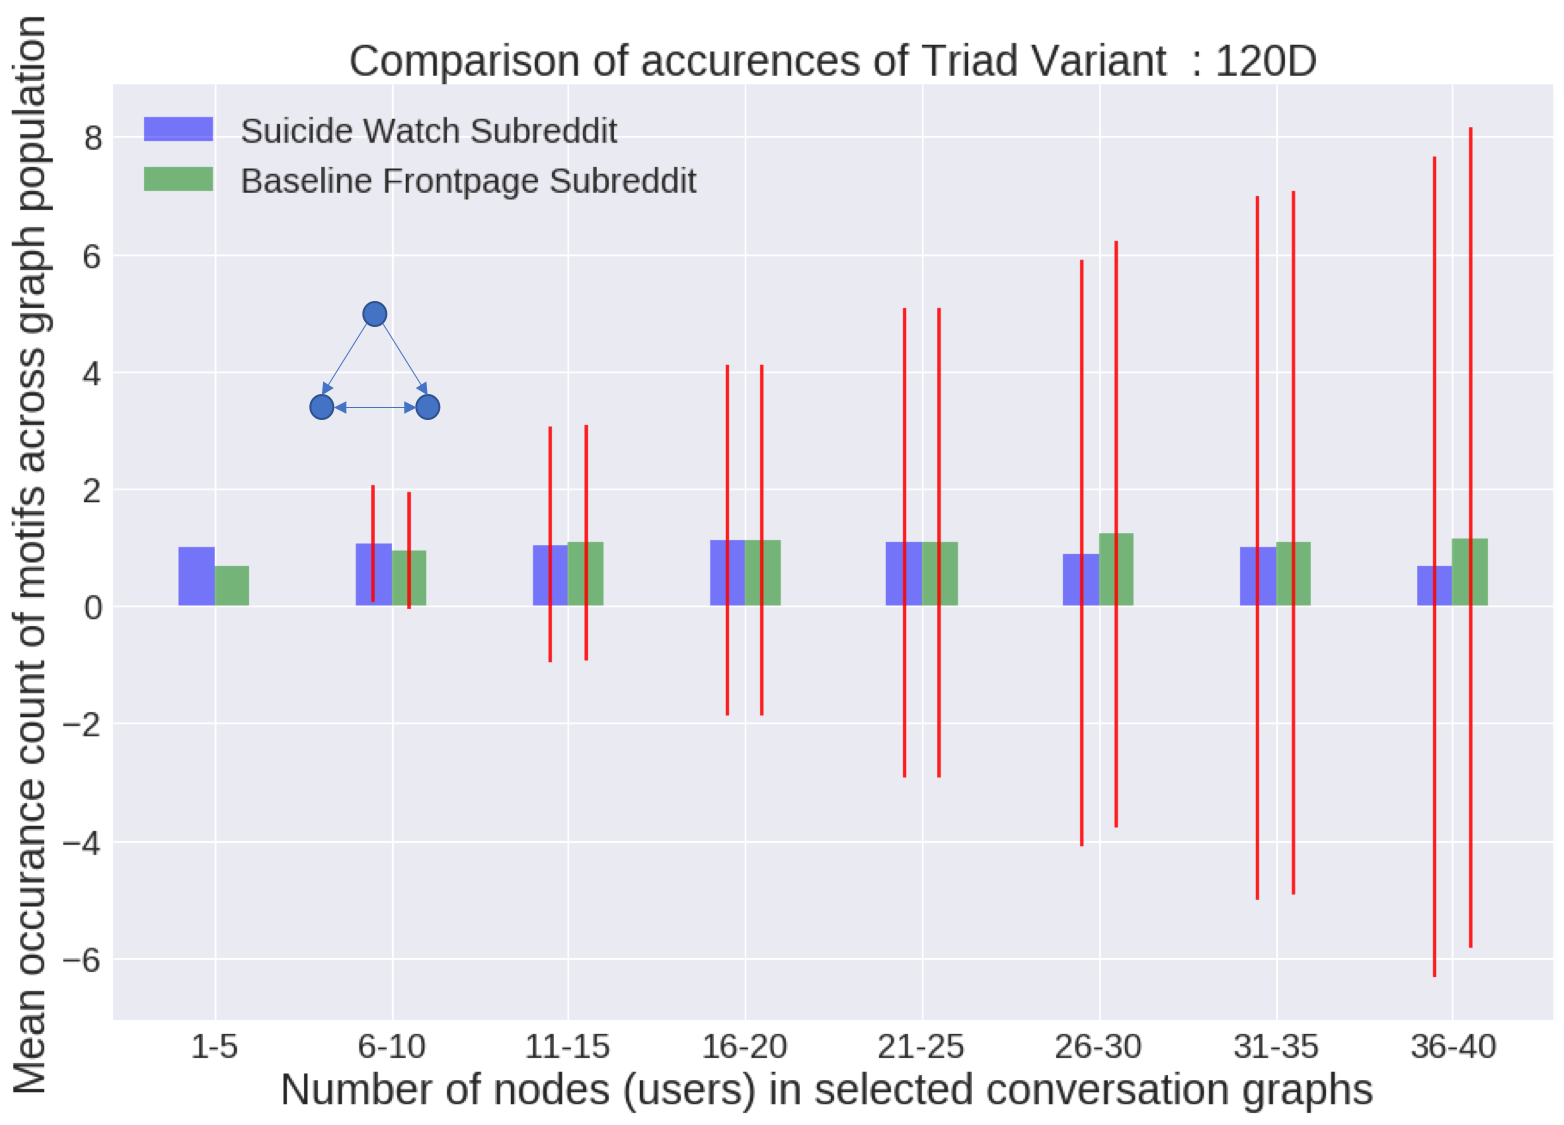
\includegraphics[width=0.33\textwidth, height = 4.5cm ]{Figures/120D}
	\label{fig:120D}
	}
    \subfloat[]{
	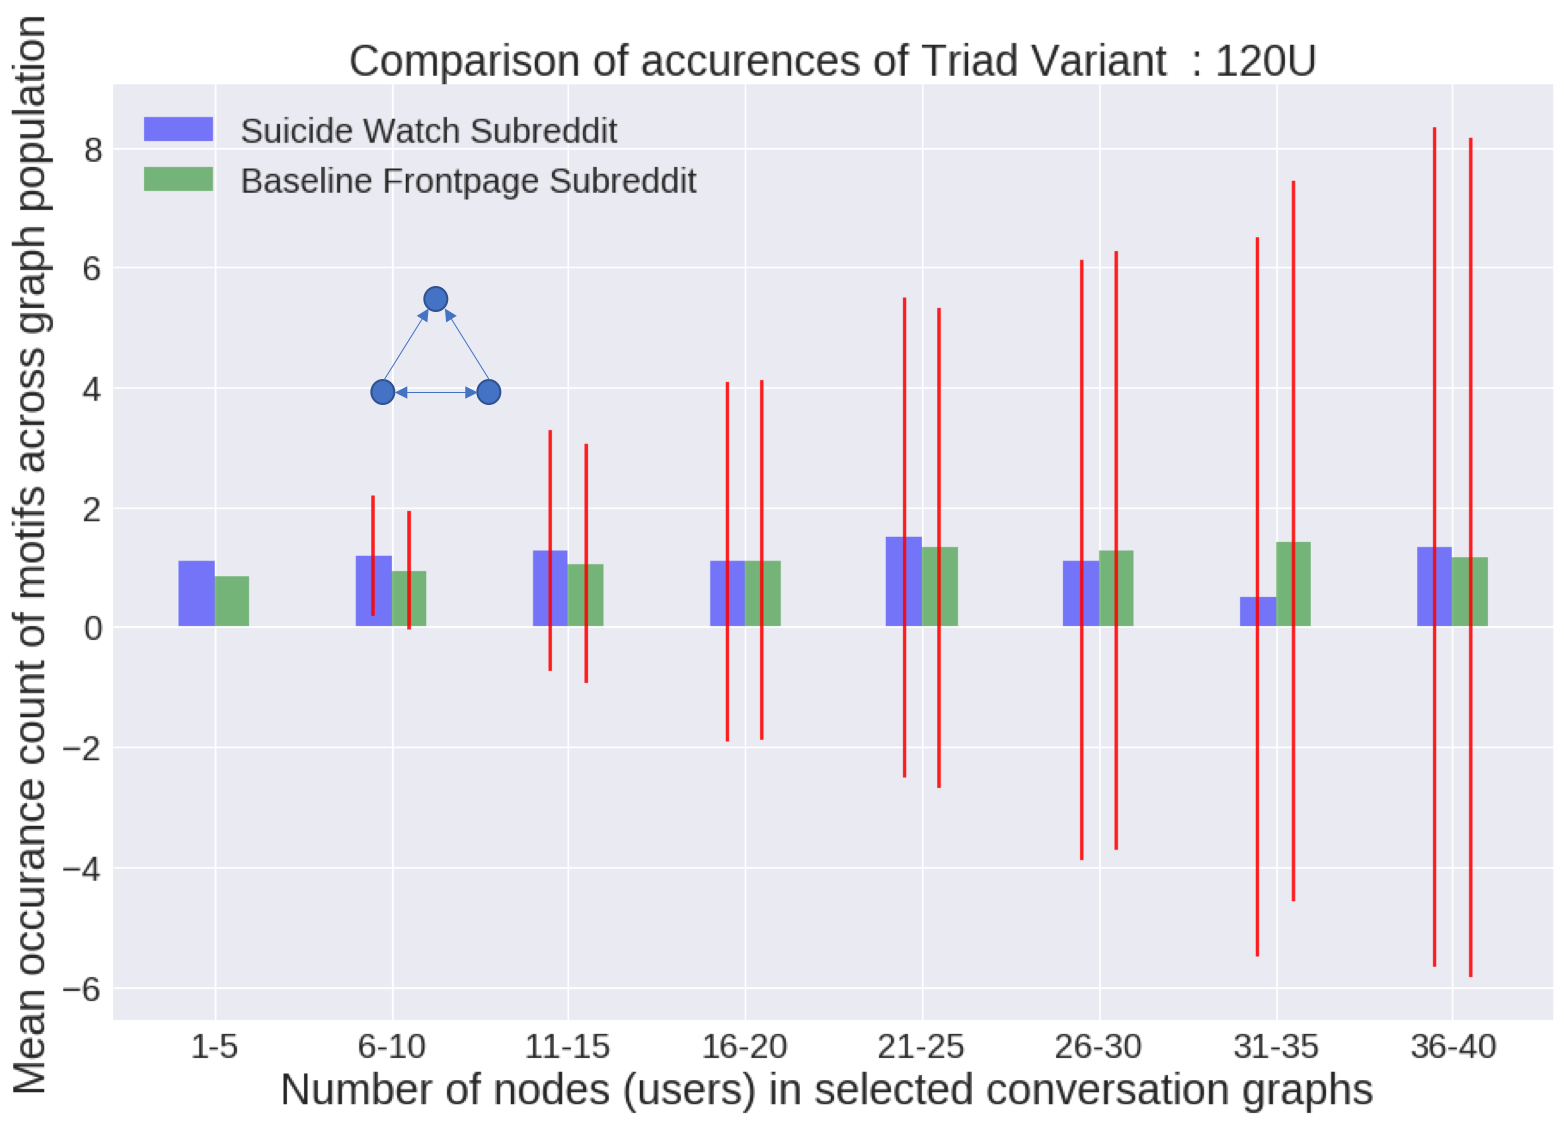
\includegraphics[width=0.3\textwidth, height = 4.5cm ]{Figures/120U}
	\label{fig:120U}
	}
    
	\subfloat[]{
	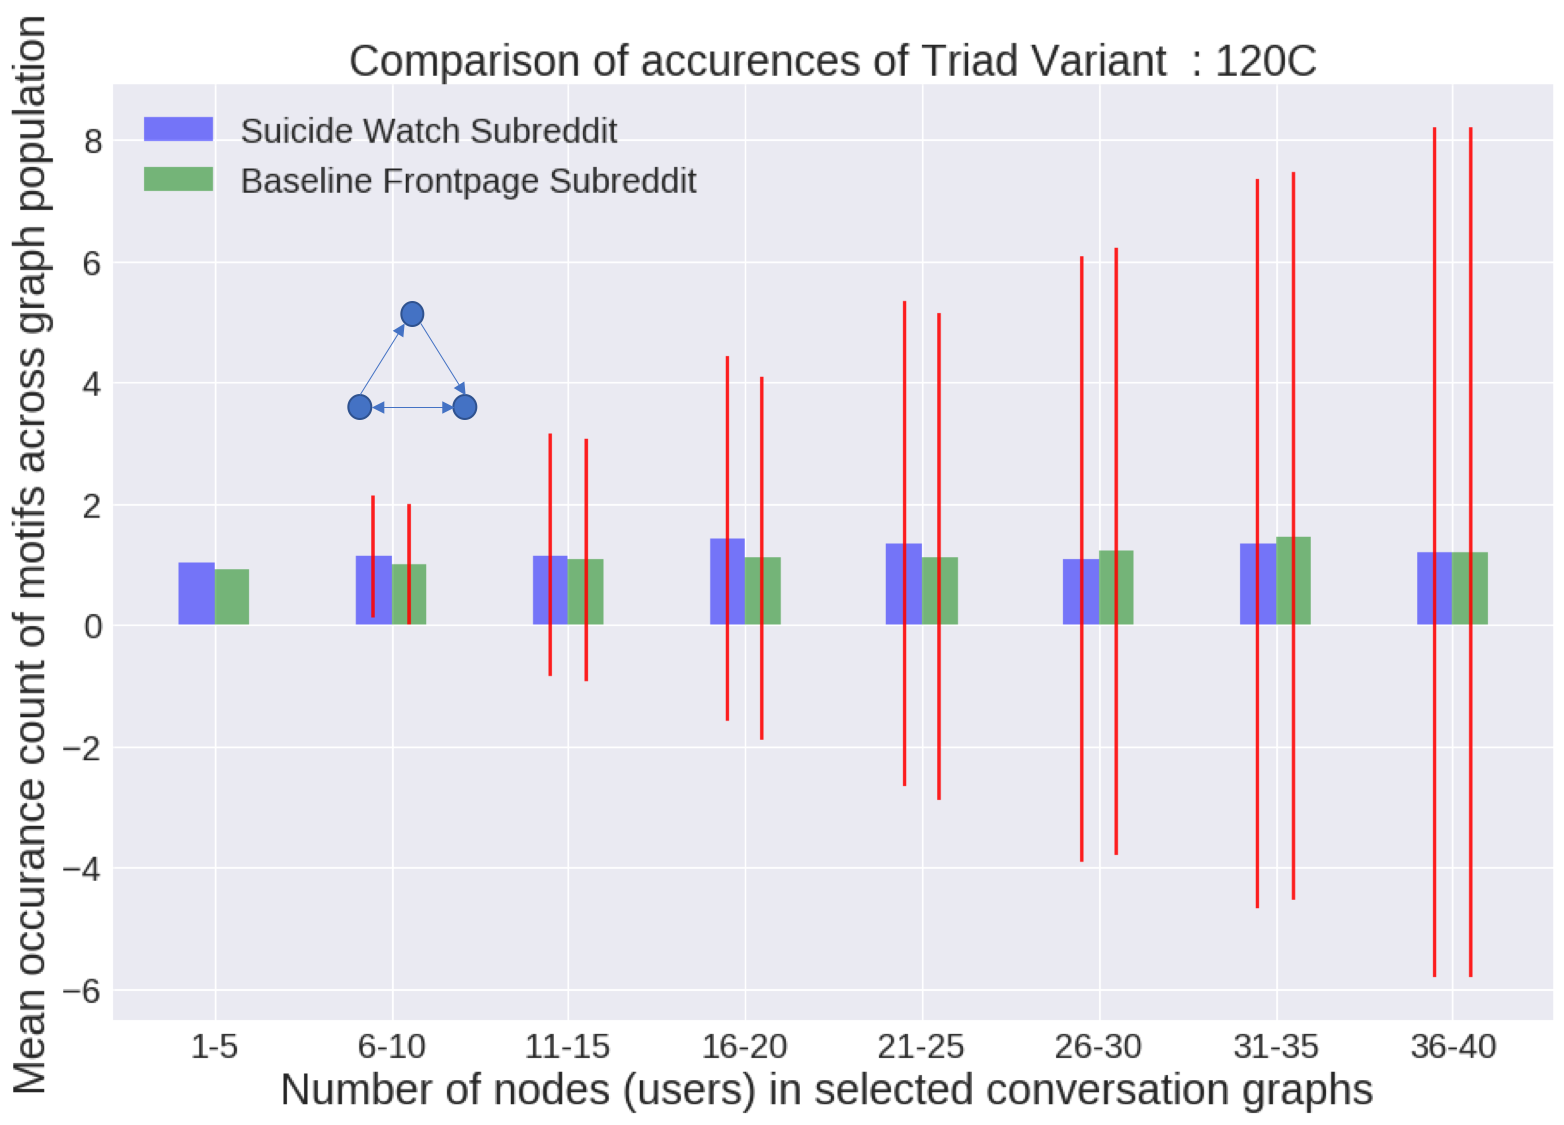
\includegraphics[width=0.33\textwidth, height = 4.5cm ]{Figures/120C}
	\label{fig:120C}
	}
	\subfloat[]{
	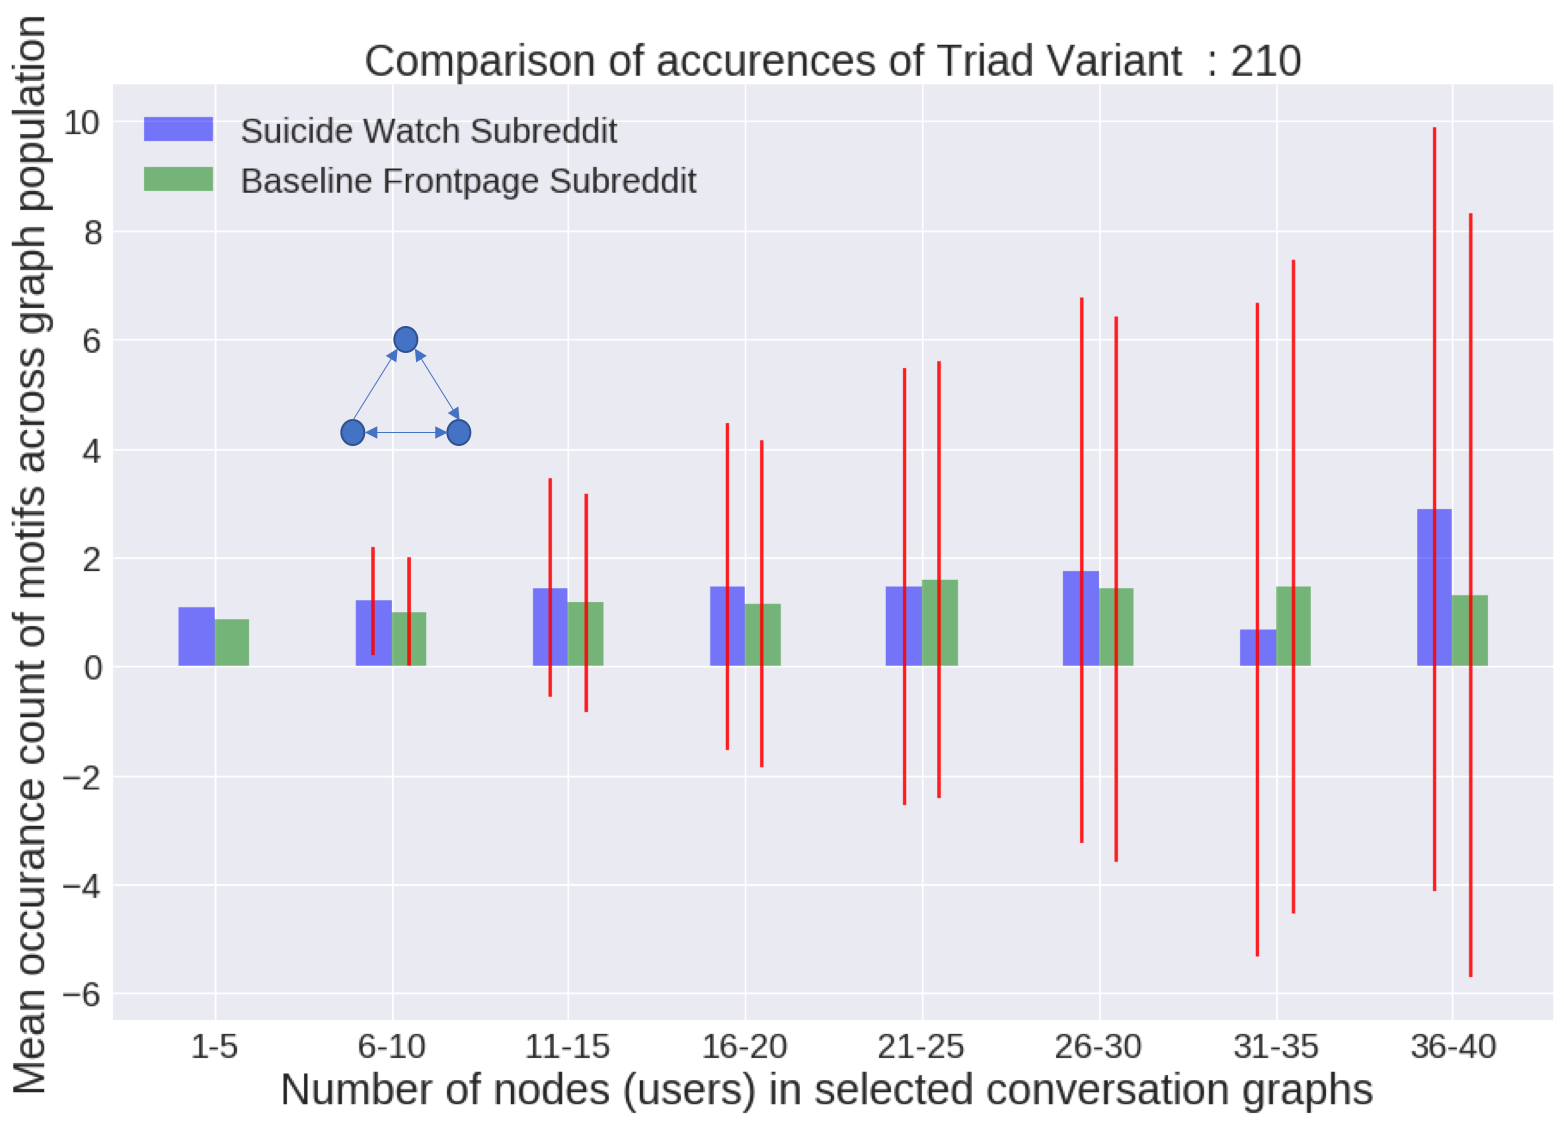
\includegraphics[width=0.33\textwidth, height = 4.5cm ]{Figures/210}
	\label{fig:210}
	}
	\subfloat[]{
	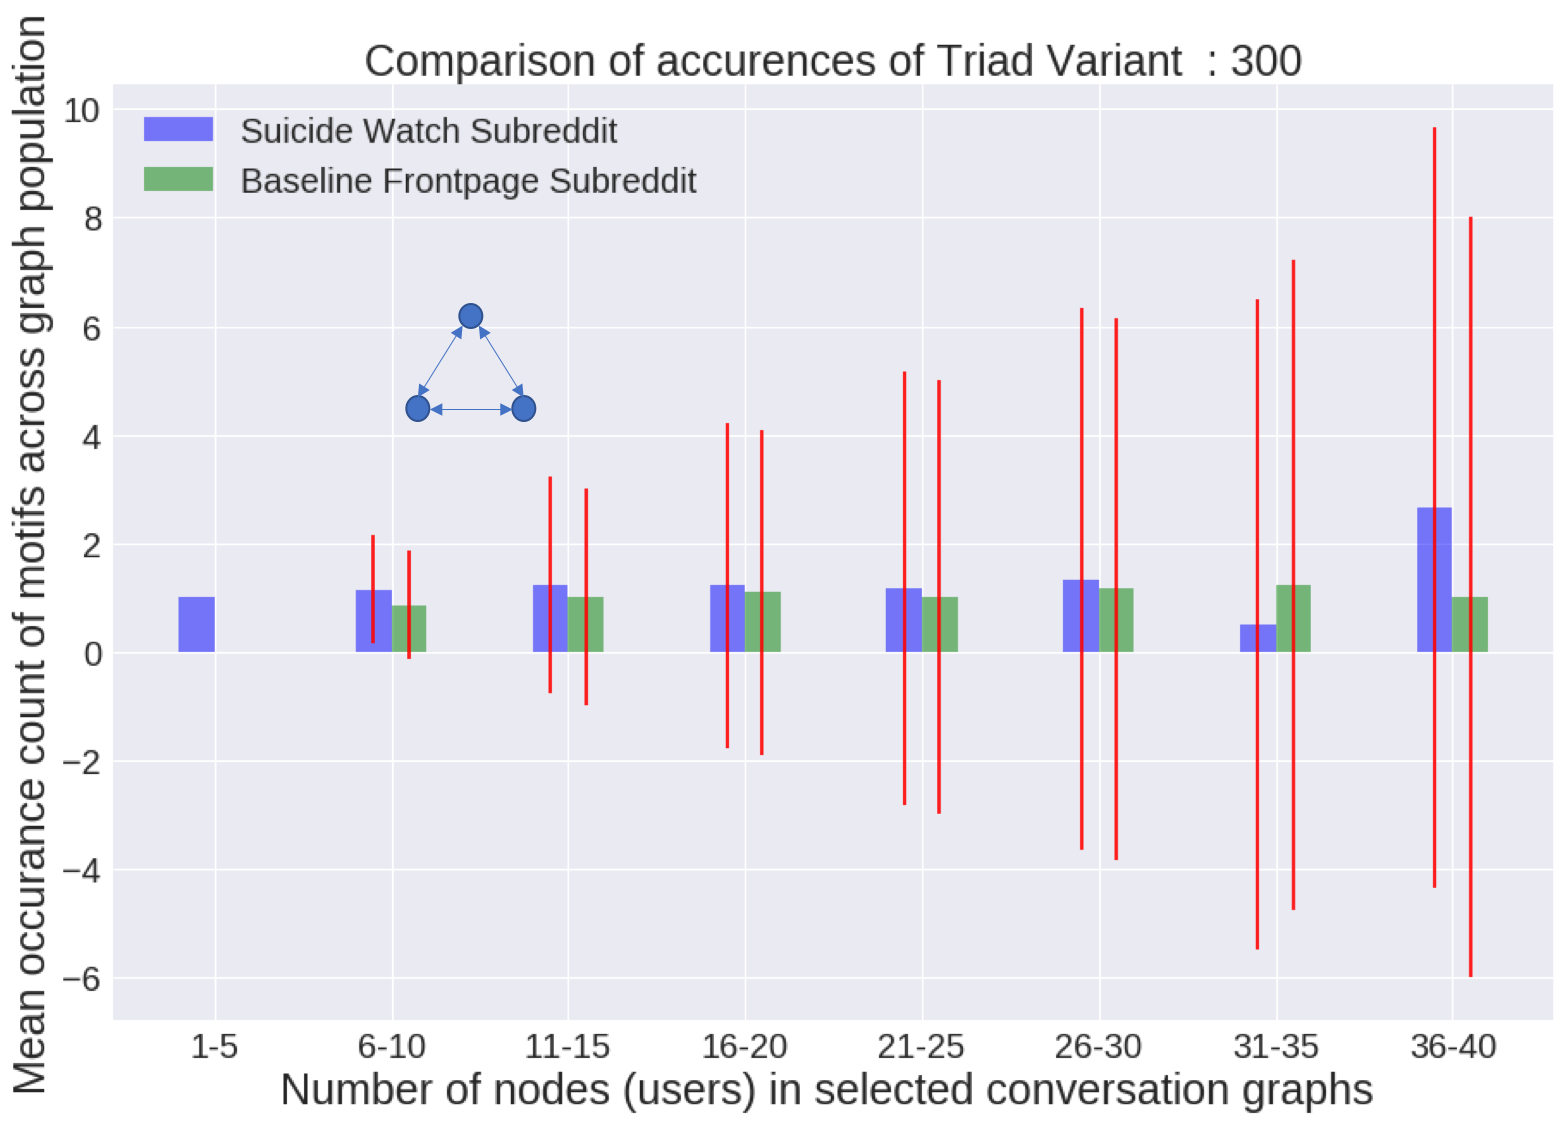
\includegraphics[width=0.33\textwidth, height = 4.5cm ]{Figures/300}
	\label{fig:300}
	}
	
	\label{fig:MotifOccurance}
	\vspace{-0.4cm}
	\caption{ The figure shows comparison of occurrence ratios of 9 insignificant motifs. Blue traces are for Suicide watch and Green traces are for Baseline Front page threads}
	\vspace{-0.4cm}
\end{figure*}